\chapter{Is It Worth Investigating?}
\label{chapter:worth}

\section{Introduction to This Research}
\label{section:justification introduction}

\todo{Incomplete}

\section{The Technology of the Web}
\label{section:the technology of the web}

The World-Wide Web (WWW, or just the Web) has become the largest information, communication and commerce system on the planet. As discussed in previous chapters, this research is concerned with the energy use of software applications and components used on the web. To provide context for the experimental work in further chapters it is important to be clear about the technology and terminology used in web systems.

\subsection{Transfer Protocols: HTTP, HTTPS etc.}
The web is a distributed system, consisting of hundreds of millions of servers and many more client devices. For all these systems to work together there needs to be standard communication and data transfer protocols. The earliest web servers used the original Hypertext Transfer Protocol (HTTP) \todo{citation}, now referred to as HTTP 1.0. later versions added extra features, authentication and security, but the core of the protocol remains the same. In this document the term HTTP will be used as an umbrella term including the various HTTP and HTTPS versions.

HTTP is a \emph{Request-Response} protocol. Communication is initiated from the client system. This client system is usually a web browser, but HTTP is just as usable from any application, such as a desktop or mobile "app", which needs to communicate with a web server.

An HTTP request is sent as plain text and consists of a series of "request header" lines followed by optional "body text". The server reads the header lines to determine what type of request it is as well as the resource it refers to, expressed as a Uniform Resource Locator (URL), and any additional information necessary to service the request. If the server cannot handle the request it returns an error response containing one of a variety of standard error codes and an optional error message. If the server can handle the request it returns a success response with a success code of 200, followed by a series of "response header" lines followed by optional "body text". In most cases it is the job of the server to populate the response headers and body with the requested information. More information about the HTTP protocol can be found in the original "Request For Comments" (RFC) \citep{Berners-Lee1996} or any of the subsequent documents.

\subsection{Servers and Websites}
The requirement to specify a resource using a URL in an HTTP request is vital, as it allows a single HTTP server to respond to requests for more than one resource. This collection of resources has become known as a \emph{website}, and each addressable resource as a \emph{web page}, even though resources can be a wide variety of types including binary resources such as images and machine-readable data formats such as JSON or CSV. Some websites have no human-readable pages at all, but instead function as an Application programming Interface (API) to some other server-side software.

Modern web server software can host multiple websites on a single server using a technique known as \emph{virtual hosts} and do a variety of other tricks such as acting as a proxy for another server. 

\subsection{Static Websites}
A website is classed as \emph{static} when its pages are unchanged between requests. This may be because they have never changed since being created, or it may be because they have subsequently been changed by a person or another external action but will remain the same until manually changed again.

Static websites are the kind which were envisaged in the original concept of the Web as a shared document repository. Static websites have both advantages and disadvantages compared with other types of website. Static websites have less work to do and so can be faster and more efficient than \emph{dynamic} websites (this area is covered in much more detail in later chapters \todo{section link}). Static websites are also much more amenable to replication and local caching, both techniques which can help to increase response speed and reduce the load on the web server and the network infrastructure. On the other hand, static websites can be clumsy to manage, particularly if they include pages whose information or styling depends on other pages. An example of this might be a blog which lists recent posts in a sidebar on every page. When a post is added, every page on the website needs to be changed.

Tools are available to help with management of static websites, and these are explored in more detail in later sections \todo{section link}

\subsection{dynamic websites}
A website is classed as \emph{dynamic} when some or all of its pages vary between requests. This may be something as simple as adding a timestamp to the page when it is served, or as complex as regenerating the complete page from scattered components and services every time it is requested. Note that for the purposes of this research it is only the page served from the server which is being considered as static or dynamic. pages can appear to be dynamic to a web user when they run JavaScript code in the user's browser. In this case, though, the processing to modify or regenerate the page is done on the user's computer rather than the server. Such client-side web applications are out of the scope of this research the same as mobile "apps" and desktop client software.

Dynamic web sites have the advantage that, as pages are regenerated or enhanced whenever they are requested, there is no need to update every page when common elements change. In the case of the blog showing the latest posts, that area of the page can be automatically populated when the page is updated for return to the requesting client. The main down-side of this dynamic behaviour is the increased processing needed to produce each page, which can result in delays, extra machine load and ultimately, extra energy usage \todo{section link}. Another down-side of dynamic pages is that they are much harder to cache and distribute for more efficient server and network usage. Any caching software needs to be aware of the variability of the pages, or risk serving incorrect or out-of date pages to clients. In some cases this is so tricky that all caching is disabled for those pages, requiring a full regeneration of the page every time.

\subsection{Caching}
In software terms, caching means taking a copy of something with the intention of providing simpler, nearer, quicker, or more efficient access. Any kind of data can be cached, but this research is mainly concerned with server-side web applications, so the discussion will concentrate on caching of web pages, in whole or in part.

Caching can take place at several points in the HTTP request-response cycle. An obvious option is caching of the whole page response after it has been sent from the server. In a complex distributed system such as the internet, this information may be cached several times. For example:
\begin{itemize}
    \item A client-side application such as a web browser can cache the page to avoid the need to re-request the page from the server if, for example, the window size is changed and the page layout needs to adjust to fit the new size.
    \item The internet access provider or local network used by the client-side application can cache the page to reduce the need to re-request the page from the server if it is needed by more than one user.
    \item A global cache infrastructure such as Cloudfront \todo{citation} can cache the page at several locations around the world to reduce long-distance network traffic
    \item The server-side application developers can add a local cache layer such as Varnish \todo{citation} or W3 Total Cache for Wordpress \citep{BoldGrid2022} which will not significantly affect network traffic, but might increase response speed and help reduce the amount of processing required by the server-side application.
\end{itemize}

Caching can certainly improve performance, particularly when generating a page is a relatively slow process. How much effect it has on overall energy consumption is still an open question, though. The energy cost of generating pages may be reduced, but any savings must be offset against the cost of managing the cache infrastructure. Caching can also be a complex process. The "cache invalidation problem" is one of the long-standing challenges of computer science \todo {citation} and if caches are managed incorrectly or inefficiently they can make the situation worse rater than better.

\subsection{"Hacks", Exploits, Security Issues and Cybercrime}

Any server which is exposed to the public internet can potentially be a target for cybercrime. If the security of a server is compromised the effects can vary from mild or merely embarrassing to much bigger problems. The impact of a compromised web-facing application or server is not limited to just the organisation operating the application, although that can be business-damaging and potentially very expensive, but if the compromised system is repurposed to aid in other attacks the damage can ripple outward to other servers, applications and organisations.

Not all web facing applications are vulnerable in the same way, though. Some applications, by dint of their complexity or the way they have been implemented, have a broader "attack surface" \todo{citation} than others. To minimise vulnerability, servers and applications need to be kept up to date with the latest security improvements, particularly when vulnerabilities are discovered in any of the third-party components which have been used to build the application \todo{cite log4j?}. This can be a complex process, requiring that anyone operating a public application be aware of the details and versions of every component used by the application.

If and when it is discovered that a server or application has been compromised, the organisation operating the system needs to act to mitigate the problem. Part of this mitigation will be immediate, and include steps such as switching off or isolating the compromised system and rebuilding or restoring from backups. Part of the mitigation will act to prevent a similar problem from happening again. This is usually a much longer, more involved, and potentially more expensive process as it can include redesigning and re-implementing the vulnerable parts of the system.

On the whole, a simpler application is probably less vulnerable \todo{citation to back this up}.

\subsection{Operating System Landscape}
Although there are some moves toward supporting "bare metal" applications on the web \todo{citation}, most mainstream web applications require the services of an operating system. The requirements of an operating system for a web server are different from that for a typical desktop or laptop computer, mainly because there is no need for usually a graphical user interface (GUI), keyboard or mouse. All communication with a server, including deploying and managing applications and communicating with users and other services is done over a network. An operating system installation without the usual GUI facilities is known as "headless" \todo{citation}. Most well-known computer operating systems are available in "server" or "headless" variants, including Windows, Mac OSX, some other Unix variants such as FreeBSD, and Linux.

Windows and MacOS operating systems are licensed and either require payment of a fee, purchase of specific hardware or some other agreement with the manufacturer. Linux and most of the other Unix variants are free and open source, which makes them a much easier choice. Linux is available in a variety of flavours known as "distributions" or "distros". For some distributions there are paid options, paid support contracts or licence restrictions, but in almost all cases the software can be installed and used for free. Linux is overwhelmingly the most popular choice for server operating systems \todo{citation}.

Linux distributions provide methods to install and update software and services from shared repositories, and the software in these services includes all the basics required to get a web application up and running such as a selection of web server software, programming languages, libraries and databases.

\subsection{Web Server Software Landscape}
The first generally-available web server software was simply known as \emph{httpd} (a contraction of HTTP daemon, where "daemon" is a slang term for a background service). Since then there have been a profusion of services and components which can server resources and respond to HTTP requests. These can be grouped into several categories:

\paragraph{Classic Web Servers}
This category includes web server applications which listen to port 80, the standard HTTP port and probably also 443, the standard HTTPS port, and will serve file resources from a nominated directory on a hard drive. Some web servers do just this, but others support a variety of extra features such as virtual hosts to serve resources from more than one domain, the ability to forward or proxy requests for another server, the ability to adjust incoming URLs and so on. Servers in this group include Apache2 \todo{citation}, NginX \todo{citation}, and Lighttpd \todo{citation}.

\paragraph{CGI and FastCGI}
The earliest attempt to add intelligent processing to HTTP requests was through the Common Gateway Interface (CGI). This is an addition to a classic web server which can recognise requests for certain resources (typically by their location in the file system or by a specific file extension) and run them as a command or script rather than merely returning the contents to the client. CGI code can be a bit clumsy  as it relies on the code being executed generating a complete valid HTTP response on its standard output stream, and supplies headers and other request information via \emph{environment variables}. CGI scripts are \emph{stateless}, which means that they must rely on other means (such as writing data to files or to a database) to store information between requests. This statelessness does, however, make them relatively easy to test.

The main disadvantage with CGI is the overhead of locating, loading and running a complete program for every request. This can be a significant overhead if the program is large or needs to wait for external resources when it starts. To solve this, the FastCGI protocol was invented. FastCGI also allows a classic web server to add dynamic behaviour, but using a different mechanism. Instead of loading and running a fresh program for every dynamic request, FastCGI passes the details of the request to a program which is already running. This is similar in concept to redirecting the request to another server, but FastCGI does not necessarily use the HTTP protocol for the internal communication. FastCGI is particularly popular with the PHP web programming language.

\paragraph{Application Servers}
Application servers can usually serve files in the same way as a classic web server, but also provide the ability to run application code without needing to run another program or pass the request to another server. When an application server receives an HTTP request which is associated with code, that code is executed directly by the application server and the result is returned in the response to the client. Application servers are usually closely associated with a particular programming language and run-time environment, and understand the semantics of mapping a request to appropriate code and data in that language. Most significantly, compared with CGI, the code associated with web resources can maintain \emph{state} between requests, such as which user is logged in or the progress of a multi-page form.

Examples of application servers include Tomcat \todo{citation} and Glassfish \todo{citation} for Java, Express for Node.js, and WSGI \todo{citation} for Python.

\paragraph{Development Servers}
As well as the "big names" in application servers, there is another large group which provide similar kinds of features, but aimed at a different purpose. These servers are intended for use while developing software, so they may not have the full range of performance features, but make up for it with easier investigation and "debugging" of problems. Development servers exist for all major programming languages. Although development servers are intended for use in a development environment, they are sometimes also encountered on the public web.

\subsection{Web Application Frameworks and Platforms}
An operating system, a web server and a way for incoming HTTP requests to be routed to some appropriate code may be sufficient for simple applications, but in many cases it makes sense to build on existing code deigned for similar uses. Such software is known by a variety of names, including a framework, a platform, or a content management system, for example. Each of these terms has slightly different implications, but essentially they are there to deal with the things which are common to many web applications, so each product does not need to design, create, and test everything from scratch.

Typical assistance provided by frameworks and platforms includes  help with interpreting HTTP requests and formatting HTTP responses, storage for information persisted between requests and a range of libraries for tasks such as communicating with other systems, accessing databases and so on. The aim of a framework or platform is usually to make the process of going from an application idea or feature to a working system as straightforward as possible. In order to achieve this, however, frameworks and platforms need to make simplifying assumptions about the kinds of things an application will need to do and the way it will need to do them. This in turn can act to restrict the things that an application written using that framework or platform can do. Frameworks and platforms which include a lot of such assumptions are colloquially known as "opinionated" \todo{citation}.

\subsection{Architecture of Web Applications}
Regardless of their specific purpose, web applications need to meet certain operational standards. Primarily they need to correctly implement the HTTP protocol, of course, but they also need to handle the real quantity of requests and then respond quickly enough. A web application may function perfectly correctly in a development or internal test environment, but that does not ensure that it will be able to handle real-world loads without errors or slowdowns.

To handle higher loads and maintain acceptable response times often requires more processing than a single server can provide, so many high-volume web applications run on a cluster of real or virtual machines working together. This has a significant effect on the architecture of the product, as it means that software can no longer automatically rely on variables in the memory of a single machine for data persistence and communication between requests. Scaling the number of collaborating servers is also vitally important. Too few will reduce the quality of the service while too many will increase the cost of providing the service. Fore some systems the load is predictable and stable enough that a fixed number of servers will suffice, while others need to "scale up" and a"scale down" the number of servers as the load rises and falls.

\subsection{Content Management Systems}
The concept of a content management system sits somewhere between a framework and a web application, consisting of a customisable application which can be configured, often with very little actual programming, to suit the desired requirements. Content management systems may include a web server, or work with an existing web server or application server. They usually provide features for the management of the pages and their content as well as the software to respond to HTTP requests with populated pages. Examples of content management systems include Zope for Python \todo{citation} and Joomla for PHP \todo{citation}. According to web statistics, the most popular content management system on the web is WordPress, also written in PHP, which serves over 40\% oi the websites in the world. \todo{citation}

\subsection{Templates and Template Engines}
Almost every use for computers has a need to produce textual output. Not just fixed, hand-crafted text but also combining such text with variable content: \textquote{a dynamic and computational 'text'} \citep{Rodgers1999}. As an example, most business software comes with some sort of "mail merge" facility for the "small print" on an invoice; a form letter with a bit more individuality than "Dear customer", and junk email offering supposedly unbeatable personalised offers.

The most common way of producing these kinds of documents uses a templating technique. A master document containing blocks of fixed text and special symbolic tokens, also known as \textquote{placeholders} \citep{Arnoldus2007} is processed through a software system which combines the supplied text with data records to produce a set of similar, but individualised, documents where the placeholders have been replaced by appropriate values from the data records.

Templating is not limited to personalised mail. A similar approach produces a \textquote{substantial fraction} of the visible pages of the web \citep{Shao-Hua2008}. In 2005 \citeauthor{Gibson2005} estimated that \begin{displayquote}Templates represent 40–50\% of the total bytes on the web, and this fraction continues to grow at a rate of approximately 6\% per year\end{displayquote}. 

\cite{Gibson2005}'s study is relatively old in technology terms. Their estimated growth has clearly not continued or by now there would be more templated content than the web itself! However, the enormous growth of the web since the study has made the determination of such estimates considerably more difficult particularly using the technique employed by \citeauthor{Gibson2005}, which relied on statistical analysis of a "snapshot" of the whole web. Despite examining over 250 papers which cite G\cite{Gibson2005}, up to and including 2017, no better estimates have yet been found.

Templated text generation is also common in much of the less visible internet traffic. Emails and other textual messages, logging, diagnostic output, code generation \citep{Fritzson2009} and many formats and protocols \citep{Barbosa2002}, all benefit from this powerful technique.

Proceeding on the assumption that templated content comprises at least \citeauthor{Shao-Hua2008}'s \citeyear{Shao-Hua2008} \textquote{substantial fraction} of the web and considering the size estimates from \cite{Worldwidewebsize2018} and \cite{Kunder2008}, the impact of differences in performance and resource usage of template software could potentially be huge.

However, it has become increasingly apparent that there is little consensus in this field. A cursory examination of the popular open source software website GitHub reveals over 5000 template engine implementations (Figure 2.1.1) and there are many others available through other routes. Selecting a template solution for a project can be a significant task.

\begin{figure}[ht!]
\centering
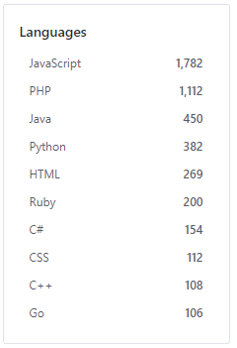
\includegraphics[width=50mm]{Figures/github_top.png}
\caption{Count of GitHub Repository matches for the term \textquote{Template Engine} as of February 2018}
\end{figure}

Comprehensive comparative information about the many differing implementations can be hard to come by. Software documentation for such tools, where present at all, tends to focus on the use of a single implementation - typically ignoring or side-lining the capabilities it lacks and avoiding direct comparison with alternatives from other providers.

This research will therefore focus on template technology as a representative category of software implementation which exhibits the scale, consequences and lack of obvious choices to be suitable for investigation. The rest of this chapter will dig deeper into template technology, its characteristics, and the range of implementations.

\subsection{Concepts and Terminology}

There are several key concepts which inform this research. The intention is to explore these in detail in further sections, but for now, some non-definitive descriptions:

\begin{description}
\item[Template] 

A template is a way of ensuring consistency and reducing re-typing when creating similar documents. Common text and layout are entered just once and then reused to produce many pages or documents. Each template is described in terms of a specific template language and designed to be rendered by a specific template engine.

\item[Template Engine] 

A template engine is a software system or component which manages the rendering of templates. When an output document is required, the template engine locates an appropriate template, loads the data for the desired document into a page context, then processes the template by interpreting it according to the template language and replacing placeholder expressions with appropriate data from the page context. 

\item[Template Language] 

A template language specifies how a template is expressed. Most template languages consist of a combination of fixed text ready for output (also known as \textquote{boilerplate}) as well as template expressions, although some template languages use symbolic expressions for everything, including fixed text. Template languages and their template expressions vary widely, but within many template languages it can be useful to consider two types of template expressions: placeholder expressions and control expressions.

\todo{Give examples of different template languages}

\item[Placeholder Expression] 

A placeholder expression is a sequence of symbols used at a location in a template which will be replaced by some external or variable text when the template is rendered. The details of the formatting and syntax of such expressions are specified as part of the template language, but the text or data which is included in the output depend on the page context.

\item[Control Expression] 

A control expression is not directly replaced by a value in the rendered output, but instead informs the process of rendering the template. Typical control expressions mimic those of conventional programming languages and include, for example: variables, decisions, and loops. Others may have side-effects specific to a particular template engine or language

\item[Page Context] 

When a template is rendered, the placeholder expressions will be evaluated to look up the data or text which will replace them. As each rendered page will potentially be different, the rendering process evaluates the template using the specific data from the page context for that page.

\end{description}

\subsection{Categories and Taxonomy of Template Systems}

There is a substantial body of literature which mentions some form of templating in passing, either philosophically \citep{Bush1945} \citep{Nelson1974} or as a means to achieve a specific end \citep{Caldwell1998} However, while these may contain useful information about the selection and use of templating systems, they are not the core of this research. The pool of literature which directly addresses theory and implementation of templates and template languages seems much smaller.

Grouping and categorising is a key way to advance knowledge. \cite{Vegas2009} assert that in science and engineering, knowledge matures as the investigated objects are classified. With the rise in popularity of template approaches, particularly when used to generate web pages, some effort has been put into trying to group template languages and/or template engines into categories to build a body of knowledge and determine unifying constructs; interrelationships; and knowledge gaps \citep{Vegas2009}, with which to reason about capabilities and applicability for different kinds of usage.

\cite{Vosloo2008} set out to survey and classify the landscape of server-side web page generation frameworks. Tellingly they are unable to find other literature at this level of detail:

\begin{displayquote}
This proliferation of discussions and solutions may be construed as an indication that the problem (of finding the right abstractions with which to implement Web-based UI) has not been solved satisfactorily in practice. However, it may also be that the problem merely has a great number of variable parts, and that it needs to be partitioned more usefully. \citep{Vosloo2008}
\end{displayquote}

\cite{Vosloo2008} initially divide the web page technologies they examine according to the three aspects of the popular MVC (Model, View, Controller) pattern. This research is primarily concerned with what \citeauthor{Vosloo2008} describe as \textquote{view concerns}. They consider possible taxonomies of page-generation strategies including various forms of templates, eventually presenting the following diagram:

\begin{figure}[ht!]
\centering
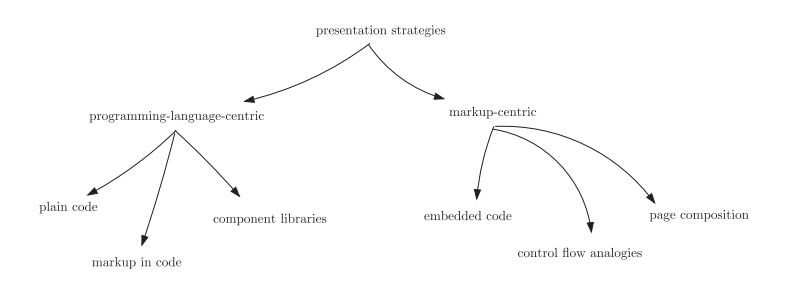
\includegraphics[width=130mm]{Figures/taxonomy.png}
\caption{A Taxonomy of Strategies for View Concerns from \cite{Vosloo2008}}
\end{figure}

The final paragraph of \citeauthor{Vosloo2008}'s \textquote{view concerns} section highlights the usefulness of taxonomy construction in finding under-considered areas:

\begin{displayquote}
"For example, none of the 80 frameworks studied relied on a template language with the same basic goal of the page composition variants (Section 5.8), but with a syntax external to the host markup language. ... The absence of such a category in the aforesaid taxonomy could perhaps be the trigger for developing just such a language." \citep{Vosloo2008}
\end{displayquote}

There are, however, two significant issues with \citeauthor{Vosloo2008}'s approach. The first is that only server-side web frameworks were considered for the study. While this does not invalidate their results, it does imply that the classification work would need to be re-done if page-generation tools in other technologies, or template techniques for non-web uses were to be included.

Another issue is a more general one with all such taxonomies. As pointed out by \cite{Usman2017} \textquote{most taxonomies are developed in an ad-hoc way}, and \textquote{taxonomies are rarely revisited, revised or extended}. New server-side frameworks and template technologies are continually being produced, and existing ones are continually being revised, updated and re-released. A several-year-old ad-hoc summary is likely to be neither exhaustive nor fully correct and should be considered as a historical source rather than a complete reference. Even with this caveat, though, \citeauthor{Vosloo2008}'s list of 86 server-side web frameworks, most of which have at least some template processing features, begins to show the scale of the problem.

\cite{Laakso2008} also attempt to categorise a selection of web frameworks. As seen in \cite{Vosloo2008}, web frameworks often have template features. \citeauthor{Laakso2008} also have trouble finding prior work on which to base their research:

\begin{displayquote}
"To the best of authors' knowledge, very little research has been done about measuring web application frameworks." \citep{Laakso2008}
\end{displayquote}

They do, however, recommend two articles: \cite{Zoio2005} and \cite{Kolesnikov2006}. \citeauthor{Zoio2005} presents a detailed and practical comparison between two frameworks: JSF \citep{Oracle2005JSF} and Tapestry \citep{Apache2018Tapestry} through the approach of building the same application twice, once in each of the two competing technologies. \citeauthor{Kolesnikov2006} describes the use of Tapestry in an MSc dissertation.

\citeauthor{Laakso2008} take an experimental approach, as does \citeauthor{Zoio2005}. Both design one or more scenarios, apply them to each of the implementations, and use the results to measure the suitability of different software systems. The comparisons generally concentrate on ease of development and deployment, although there is some mention of rendering performance, which may be analogous to efficiency, and thus affect resource usage. 

Concentrating more specifically on templates, \cite{Parr2004} sets out to 

\begin{displayquote}
"formalize the study of template engines, thus, providing a common nomenclature, a means of classifying template generational power, and a way to leverage interesting results from formal language theory." \citep{Parr2004}
\end{displayquote}

\citeauthor{Parr2004}, however, presents the opinion that a template is a pure and separate view and should be "totally divorced from the underlying data computations whose results it will display" (ibid p2) While this is arguably a justifiable position, it does lead to a taxonomy which essentially has two categories: those which enforce separation, and those which do not. The fully separated category mainly consists of a new template language (\textquote{StringTemplate}) developed alongside the paper, with almost every other solution relegated to \textquote{do not}. \citeauthor{Parr2004} also limits his discussion to template-style solutions written in the Java programming language.

Although \citeauthor{Parr2004}'s StringTemplate language has been used for other academic publications \citep{Fritzson2009} \citep{Arnoldus2010} \citep{Hartmann2011} \citep{Arnoldus2012} \citep{Vollebregt} and many more, Parr admits that commercial programmers often prefer the features of other, less pure but more powerful, template languages. Implicitly, therefore, there is still a need to categorise these other template languages beyond simply whether they enforce separation.

\cite{Arnoldus2010} also addresses the language used in templates, but from a grammatical perspective. The important categorisation distinction in Arnoldus’ work is that of \textquote{safety}. Having determined that \textquote{Writing templates, and code generators in general, is a complex and error prone task} (p103), Arnoldus introduces the concept of a \textquote{syntax-safe} template, which is incapable of generating grammatically incorrect output This is particularly important when the output is intended to be machine readable, with a formal grammar, and Arnoldus concentrates on the specific application area of program generation, which exhibits these characteristics. Although Arnoldus does not attempt a categorisation of template languages, he does discuss several key factors (such as the presence of \textquote{hedges} (p111)) which are commonly found in those template languages which are more suitable for syntax-safe applications.

\subsection{Discussion}

Templates are the technology of choice for a large proportion of the world's web pages, and thus it seems plausible that the generation and transport of these pages contributes in some part to the large energy and resource usage of the internet and the world wide web.

While there has been some consideration of template engines and template languages in academic literature, the quantity of such papers is dwarfed by the number of software implementations, websites and documentation which have not been through an academic peer review process. Attempts have been made to construct taxonomies in related fields such as web applications, and crowd-sourced information is available from sources such as Wikipedia, but so far, no sign has been found of a detailed and comprehensive comparison and analysis of a wide range of template engine implementations.

It would seem, therefore, that there is an opportunity for research in this field to contribute to knowledge and also to potentially assist in improving the overall resource usage of large software systems.

            * Characteristics of Template Languages
            * Characteristics of Template Engines
            * Discussion

\section{The Literature Landscape}
\label{section:template literature landscape}

\todo{Incomplete}

\subsection{Literature Selection}

\subsection{Experimental Literature}

\subsection{Models and Theory}

\subsection{Educational Literature}

\subsection{Sociological and Psychological Approaches}

\subsection{Grey literature and Anecdotal Evidence}

\section{Methodology}
\label{section:feasibility methodology}

\todo{Update for 2022}

\subsection{Introduction}


Even though there are many implementations of template engines mentioned in the literature, there are considerably more available than can easily be dealt with in this document, and probably more than can be dealt with in a single PhD. Rather than attempt to gather detailed information about every possible software candidate before starting, the intention is to proceed incrementally, building a collection of data on a growing subset, then using preliminary analysis and reflection to inform further research until theoretical saturation.

Before embarking on a potentially lengthy experimental process, it seems prudent to attempt to determine whether such research is likely to provide interesting results. The overall research goal is to help software developers make smarter choices about the broader, long-term impact of their work, so a reasonable first step might be to look for differences in such an impact between a small selection of software libraries. This initial feasibility study will inform the structure and progress of later research.

With thousands of template engines to choose from it is important to systematically reduce the scope of any initial feasibility study. Options include limiting the study by popularity, by application domain, by the systems used by a specific cohort of software developers, by programming language, by template language, by price or many other factors. Each of these options has theoretical advantages and disadvantages, but for an initial feasibility study the emphasis needs to also be on practicality, to provide results as soon as possible to enable further decision-making.

\subsection{Selection of a Programming Language}
\paragraph{TIOBE}
\paragraph{Personal Familiarity}

\subsection{Selection of Template Engines}
\paragraph{mentions on the web}
\paragraph{Mentions in literature}
\paragraph{Some of my own}

\todo{Update to new structure}
\subsection{Construction of a Feasibility study}
\paragraph{Selection of features and test Cases}
\paragraph{Wrap each engine to conform to a consistent interface}
\paragraph{run each test a large number of times to average out "background noise"}

\subsection{Implementation of the Feasibility study}
\paragraph{Wrapper details}
\paragraph{Tracking time and success/failure}
\paragraph{Exclude first run}

Having decided to perform a feasibility study to gather preliminary data about the scope of the problem, the next phase was to design the study. Following the approach used by \cite{Laakso2008} and \cite{Zoio2005} a feasibility study was planned which would select a small number of template systems and construct a software test harness to run an identical set of tests independently on each of the systems. There was no attempt to be exhaustive with the selection of systems to test. With potentially thousands to choose from this was not deemed an appropriate use of time at this stage in the research.

The aims of the feasibility study were twofold: to ascertain if this would be a reasonable and useful approach for identifying and comparing template systems, and to establish an initial idea of the variability in features and performance between a sample of available template systems. Throughout the construction of the study, efforts were made to avoid or constrain "scope creep" \citep{Heinze2014}. The intention at every stage being to obtain useful results as soon as possible, to shape further research.

To obtain results which could more easily be compared, it was decided to limit the feasibility study to include only template systems in a single programming language. The language Java \citep{Oracle2018Java} was chosen for several reasons. Java is generally considered to be the most popular programming language in the world \citep{Tiobe2018}. Java development tools are also available at University of Suffolk and familiar to the researcher, reducing the need for training before commencing the study.

The next stage was to select an initial set of template engines for the feasibility study. StringTemplate \cite{Parr2004} has been cited several times in academic literature; Velocity \citep{Apache2018Velocity} and FreeMarker \citep{Apache2018FreeMarker} are popular in lists of Java template engines on the web \citep{Dzone2016}; Mustache \citep{Mustache2018} is probably the most widely implemented template engine, with implementations in at least 45 Languages. Four further template engines (\cite{Casper2018}, \cite{Hapax2018}, \cite{Jangod2018} and JMTE \citep{HubSpot2018} were included after examining their source code, as they take somewhat differing approaches compared to the systems mentioned above.

Two further template engines (\cite{Stringtree2018} and Solomon) were included as a baseline for comparison. Both these implementations resulted from previous personal research in this area and so provide familiar implementations to use when developing experiments and test harnesses.

With ten template engines selected it remained to design experiments to compare them. Keeping the feasibility study aims in mind, the following eight simplified \textquote{real world} scenarios were constructed:

\begin{description}
\item[Scenario S0: No substitutions (\textquote{control} case)] \hfill

The job of a template engine is to read and combine a template with some variable data by replacing placeholders. However, not all template documents contain placeholders. Some are just documents to be served unchanged. However, the processing within the template engine will likely add some overhead. This scenario will give some indication of the processing overhead in each implementation.

\item[Scenario S1: A single textual substitution] \hfill

The simplest active case for a template engine is the identification of a placeholder and its replacement with a single constant textual value. The purpose of this scenario is to evaluate the performance of this common activity.

\item[Scenario S2: A collection of textual values] \hfill

A step up from a single value is the substitution of a collection (such as an array, a list, or some other iterable object) of textual values. This scenario requires the template engine to determine in some way that the value to be substituted is a collection, and to make some attempt at rendering the contents in order.

\item[Scenario S3: A collection separated by commas] \hfill

It is usual in English when presenting a list to separate the items with commas. Given the list (\textquote{ham} \textquote{eggs} \textquote{chips}) it might be typical to present it as \textquote{ham, eggs, chips} (or even \textquote{ham, eggs and chips}, but that is less common in dynamically generated documents, and beyond the scope of this feasibility study). This scenario is an interesting challenge for a template engine, which is why it is a separate test from simply rendering the contents of a collection. Some template engines find it tricky to avoid placing an excess comma after the final item, for example.

\item[Scenario S4: Include another template] \hfill

Structural Decomposition (colloquially known as \textquote{divide and conquer}) is a key practice of software engineering, and also applies to the design and construction of documents such as web pages from component parts. For this to work, a template system must be able to include within its output the result of processing another template. This can sometimes be accomplished by pre-processing the text to be included, but that can require multiple passes to generate a single final document. This scenario evaluates the effectiveness of a template system at constructing such compound documents

\item[Scenario S5 and S6: Show a value if a boolean value is \emph{true} or \emph{false}] \hfill

Conditional execution is another key aspect of software. In the case of template processing it is a common requirement to convert a true/false value from the data to some text for display. A single word such as \textquote{yes} in a table or checklist, or an optional swathe of boilerplate, the process is the same: if the value is true, show the specified text. Of course, there is then the question of what to do if the value is false, which is why there are two tests for this scenario. Some template languages make a big issue of the difference between showing some text if true, but nothing at all if false, and showing alternative text (such as \textquote{yes} or \textquote{no}) for true or false values. These scenarios evaluate the effectiveness of a template system at converting boolean values.

\item[Scenario S7: Call some code] \hfill

Although \cite{Parr2004} considers this a "violation" of the principle of separation of logic from display, many template systems support the execution of arbitrary code during the rendering of templates. Techniques for achieving this vary widely, but with the Java ecosystem there is a standard way of invoking code from other contexts: the \textquote{JavaBean} Application Programming Interface (API) \citep{Oracle2018JavaBean}. Use of the JavaBean API allows systems such as template engines to discover and invoke code without it being compiled in to the template engine. Typical uses for this facility include showing rapidly changing data, or data which is expensive to calculate but may not be known in advance. This scenario evaluates the effectiveness of a template system at calling such external code.

\end{description}

\subsection{Implementation of a Feasibility Study}

One of the characteristics which separate template systems is the variation in their template languages. An implication of this is that templates cannot usually be re-used to evaluate different template engines. Likewise, template engines provide a variety of software interfaces.

For best compatibility of test results tests should be as similar as possible, yet the nature of the different template engines requires many differences in implementation. To resolve these tensions, an architecture was chosen which used the strategy pattern \citep{Gamma1994} to enable isolation of specific differences between the code for the various template engines.

\begin{figure}[ht!]
\centering
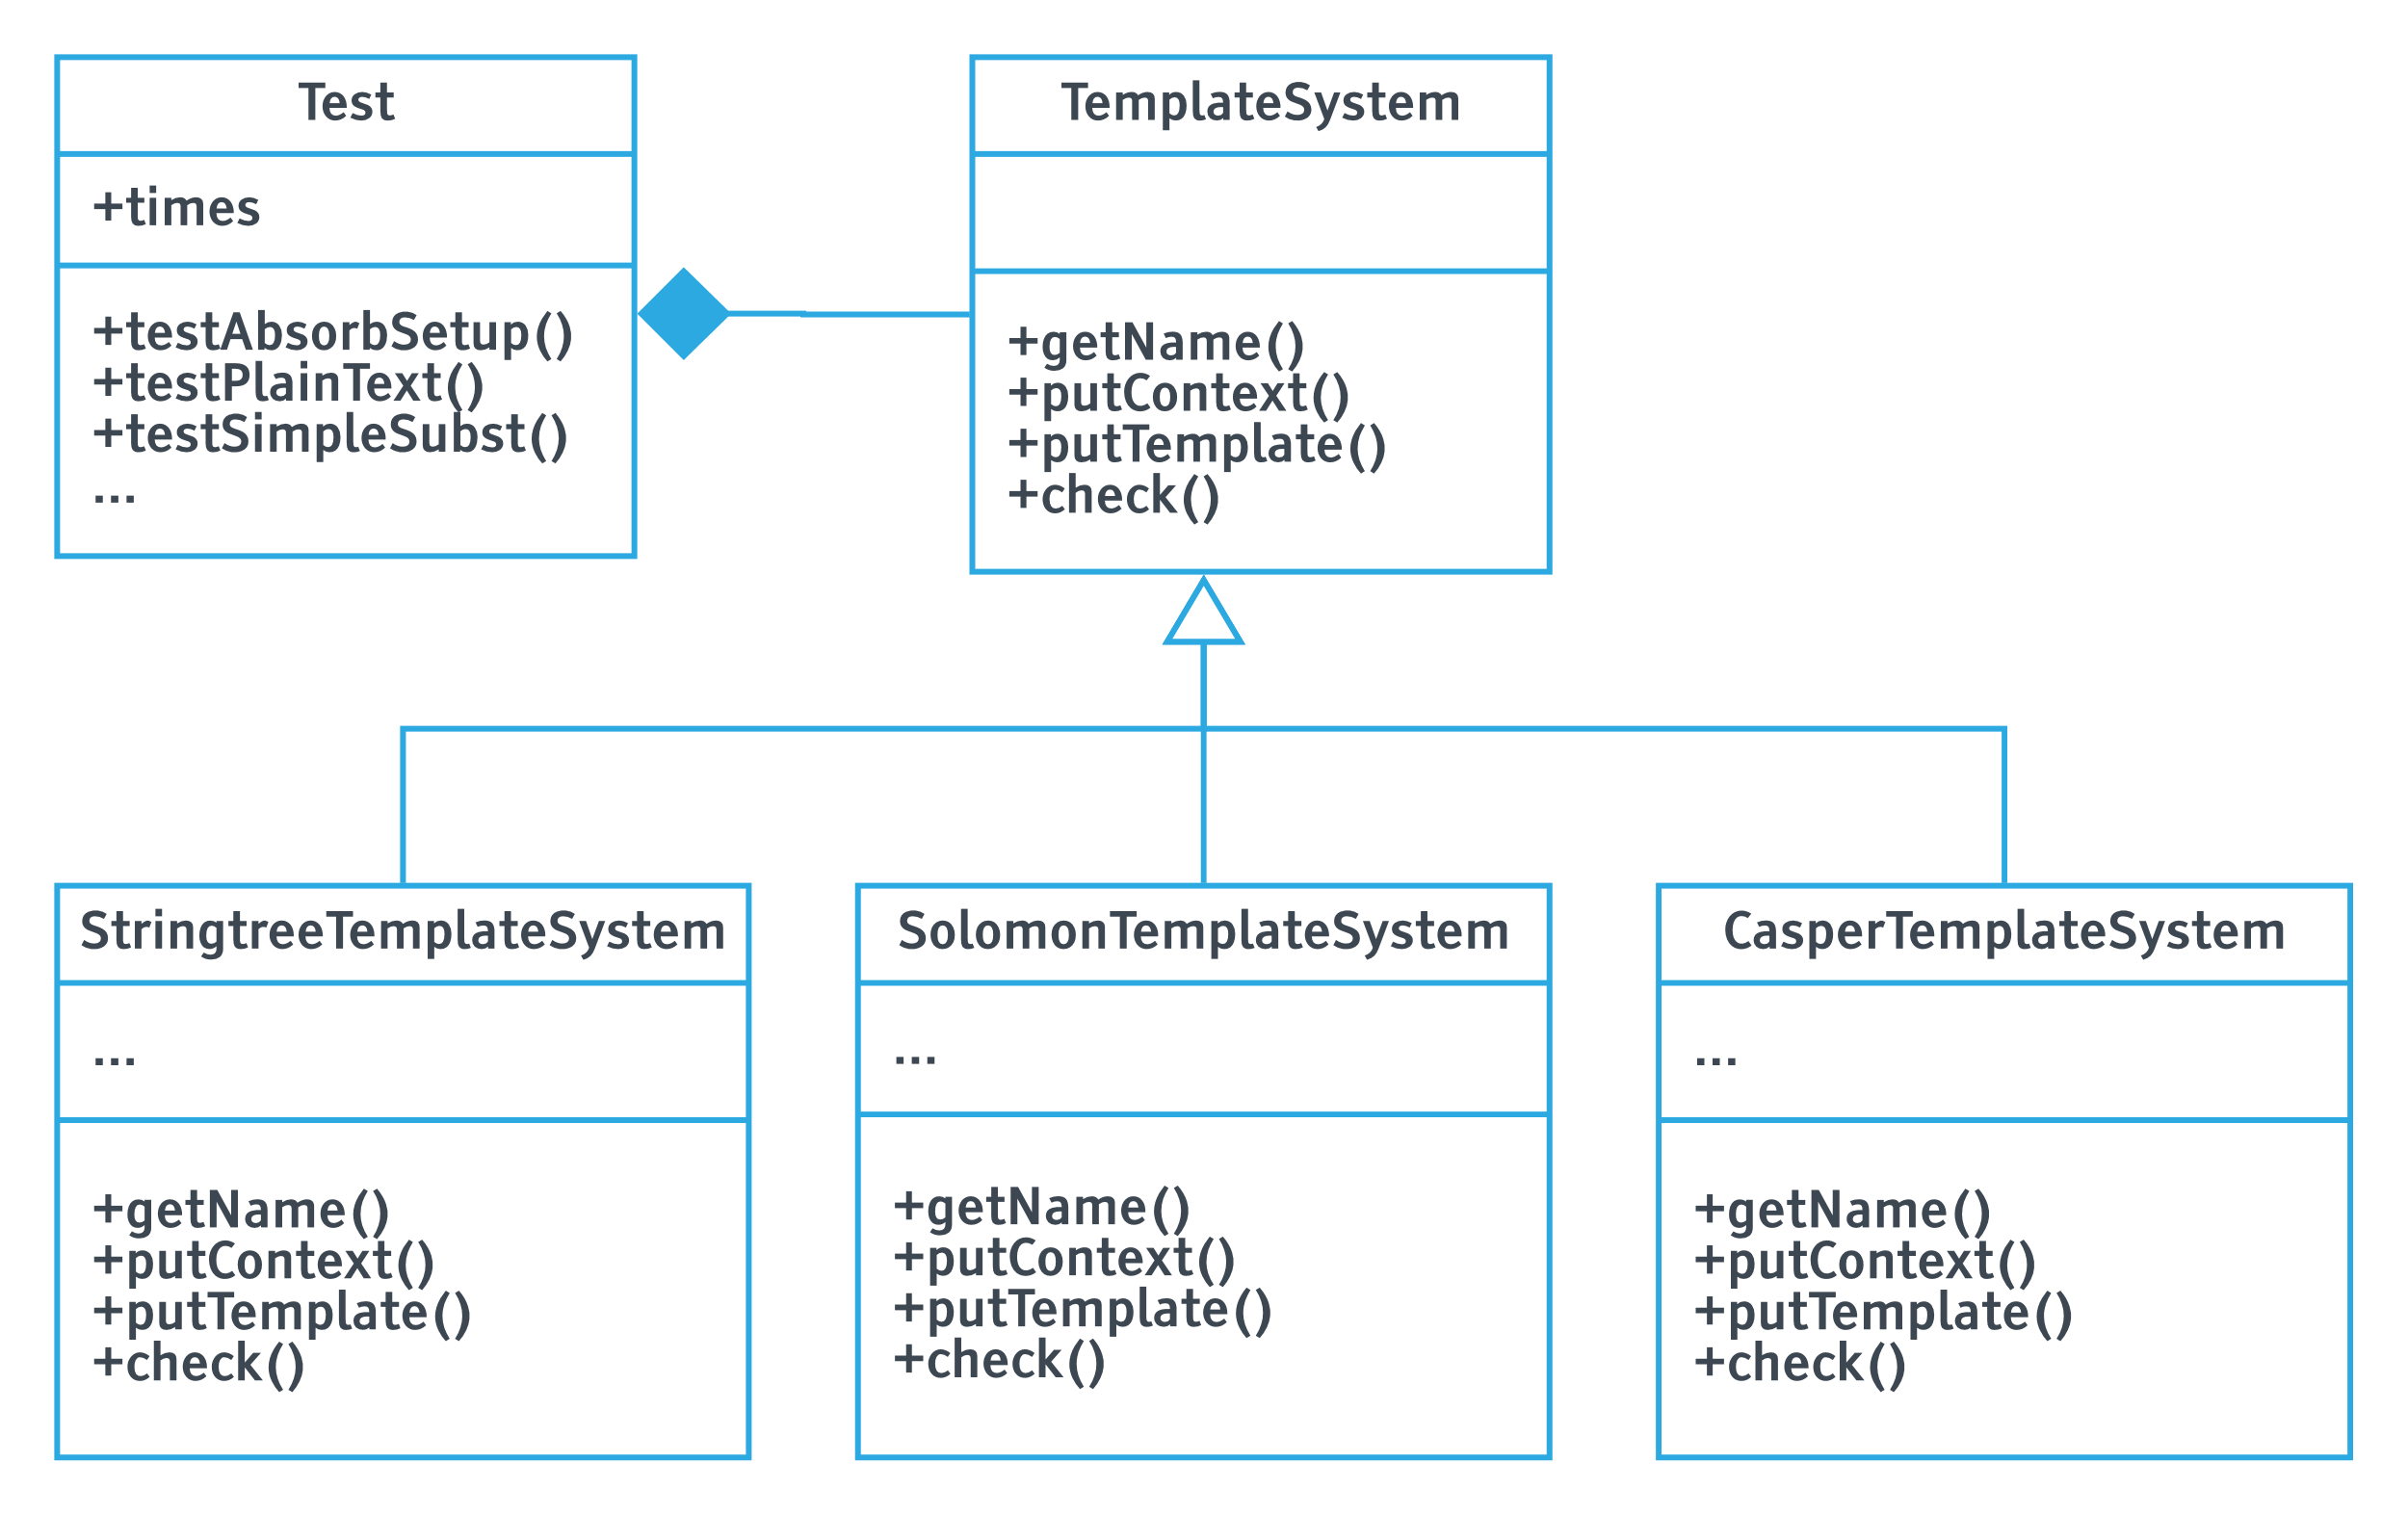
\includegraphics[width=130mm]{Figures/classes.png}
\caption{Class diagram showing use of strategy pattern}
\end{figure}

As each concrete strategy class was coded and tested, it was integrated with a test harness written using the \cite{JUnit2018} test library. When all implementations were complete, code was added to compare generated output with expected output from each test for each test harness, and to time multiple runs of each such test. Tests were timed using the Java \verb!System.currentTimeMillis()! method, which uses the system \textquote{wall clock} rather than attempting to measure only time used by specific processes or threads.

The code for the test harness underwent several changes as the template implementations were added. Most commonly this was due to differing assumptions between implementations. For example, many template engines expect to fetch templates from a local file system but some prefer other means, so the abstract definition of the strategy implementations had to change to support a wider variety of such sources. As much as possible, however, such changes were kept in the common part of the code rather than being duplicated in template-specific classes.

Despite copious reading of documentation, source code and web articles, it was not possible to coerce all template engines to generate the correct output for all test scenarios. Such \textquote{failures} are noted in the results but it was decided not to exclude these test scenarios from the timed tests.

As testing progressed it became apparent that performance of the differing template engines varied widely, so the timed part of the experiment was tuned to give largely repeatable results in a reasonable time. Eventually a value of 10,000 repetitions was settled on as an effective number. This gave largely repeatable results for each template engine.

\section{Results and Analysis}
\label{section:feasibility results}

The success of the test scenarios is given in Table 3.1, and the timings for 10,000 runs of each scenario are given in Table 3.2.

\begin{table}[ht!]
\fontsize{9}{11}\selectfont
  \begin{center}
    \begin{tabular}{r|l|l|l|l|l|l|l|l}
      & {\rotatebox{90}{{\textbf{No Subst}}}} 
      & {\rotatebox{90}{{\textbf{Single Text}}}} 
      & {\rotatebox{90}{{\textbf{Collection}}}}
      & {\rotatebox{90}{{\textbf{Separated}}}}
      & {\rotatebox{90}{{\textbf{Include}}}}
      & {\rotatebox{90}{{\textbf{Bool True}}}}
      & {\rotatebox{90}{{\textbf{Bool False}}}}
      & {\rotatebox{90}{{\textbf{Call Code}}}}\\
      \toprule
      \textbf{Solomon} & \checkmark & \checkmark & \checkmark & \checkmark & \checkmark & \checkmark & \checkmark & \checkmark\\
      \textbf{Stringtree} & \checkmark & \checkmark & \checkmark & \checkmark & \checkmark & \checkmark & \checkmark & \checkmark\\
      \textbf{JMTE} & \checkmark & \checkmark & \checkmark & \checkmark &  & \checkmark & \checkmark & \checkmark\\
      \textbf{Mustache} & \checkmark & \checkmark &  &  & \checkmark & \checkmark & \checkmark & \checkmark\\
      \textbf{Stringtemplate} & \checkmark & \checkmark & \checkmark & \checkmark & \checkmark & \checkmark & \checkmark & \\
      \textbf{FreeMarker} & \checkmark & \checkmark & \checkmark & \checkmark & \checkmark & \checkmark & \checkmark & \checkmark\\
      \textbf{Velocity} & \checkmark & \checkmark & \checkmark &  & \checkmark & \checkmark & \checkmark & \checkmark\\
      \textbf{Hapax} & \checkmark & \checkmark & \checkmark &  &  &  &  & \\
      \textbf{Casper} & \checkmark & \checkmark & \checkmark & \checkmark & \checkmark & \checkmark & \checkmark & \checkmark\\
      \textbf{Jangod} & \checkmark & \checkmark & \checkmark &  & \ & \checkmark & \checkmark & \\
    \end{tabular}
  \end{center}
\caption{Test successes by template engine and scenario}
\end{table}

It is reassuring that all the template systems in the study were capable of processing both plain text (S0) and simple substitution (S1) cases. However, these were the only scenarios which everything passed. For all the other test cases there was at least one template engine which could not manage it. Given that these scenarios were chosen as representative of common situations in professional software development, it is surprising that there was so much variability in features. The documentation for all the implementations makes some kind of claim of being "powerful" or "suitable" for a wide range of projects. 

Consider, for example, the Hapax template system which fails five of the eight tests. Its documentation states:

\begin{displayquote}
Hapax is a simple but powerful text templating library for Java. Hapax is suitable for constructing text output from Java code. The syntax is similar to Google's ctemplate library, and emphasizes the separation of logic from presentation. Hapax was designed to be easy to use and have minimal dependencies. Hapax does not depend on any existing web framework, and is suitable for use in servlets, scripting languages (Scala, Groovy, etc), and server-side applications. \citep{Hapax2018}
\end{displayquote}

Nowhere in this does it mention any limitations, making comparing implementations on documentation alone a tricky proposition. Attempts have been made to compile comparative lists of such software by features \citep{Wikipedia2018} but interpretation of the exact meaning of each feature can be loose, and there would potentially be great benefit in defining a comprehensive set of such benchmark scenarios which could be used to compare and evaluate even software which is not found in such lists.

In many cases the limitations of the template engines seem closely tied to the choice of template language. The minimalist language common to many Mustache implementations, for example, deliberately avoids constructs such as loops and conditions, in favour of performing such logic in application code before invoking the template engine. While this can be a workable strategy, it also has some potential drawbacks. It requires extra processing in the application code, which partially disguises the processing cost of generating pages compared to more competent template engines. It also requires that every possible configuration of data for the page is pre-calculated, denying the template engine any possibility of automatically re-using intermediate values or using "lazy evaluation" strategies to avoid calculations which are not eventually used. These problems become considerably more significant if the same application code is used to evaluate a wide variety of templates, each with different data requirements. In common with many software development habits, it can be easier for developers to produce code to pre-calculate everything required by every possible template, even though many of those calculations will not be required for any given rendered page. This can add extra, unneeded processing cost to every page.

\begin{table}[ht!]
\resizebox{\textwidth}{!}{
    \begin{tabular}{r|r|r|r|r|r|r|r|r|S}
      & {\rotatebox{90}{{\textbf{No Subst}}}} 
      & {\rotatebox{90}{{\textbf{Single Text}}}} 
      & {\rotatebox{90}{{\textbf{Collection}}}}
      & {\rotatebox{90}{{\textbf{Separated}}}}
      & {\rotatebox{90}{{\textbf{Include}}}}
      & {\rotatebox{90}{{\textbf{Bool True}}}}
      & {\rotatebox{90}{{\textbf{Bool False}}}}
      & {\rotatebox{90}{{\textbf{Call Code}}}}
      & {\rotatebox{90}{
        \textbf{\emph{Average}}
      }}
      \\
      \toprule
      \textbf{Solomon} & 4 & 4 & 17 & 2 & 8 & 7 & 2 & 20 & \textbf{8}\\
      \textbf{Stringtree} & 133 & 62 & 119 & 77 & 109 & 83 & 56 & 53 & \textbf{86.5}\\
      \textbf{JMTE} & 9 & 13 & 46 & 3 & 30 & 10 & 9 & 11 & \textbf{17.4}\\
      \textbf{Mustache} & 396 & 275 & 631 & 461 & 453 & 361 & 377 & 396 & \textbf{418.8}\\
      \textbf{Stringtemplate} & 239 & 243 & 322 & 150 & 350 & 158 & 92 & 40 & \textbf{196.6}\\
      \textbf{FreeMarker} & 25 & 17 & 29 & 34 & 40 & 22 & 37 & 28 & \textbf{29}\\
      \textbf{Velocity} & 252 & 168 & 282 & 250 & 205 & 178 & 124 & 114 & \textbf{196.6}\\
      \textbf{Hapax} & 64 & 79 & 124 & 58 & 117 & 43 & 49 & 55 & \textbf{73.6}\\
      \textbf{Casper} & 19311 & 15878 & 23783 & 18226 & 27997 & 21292 & 21572 & 21048 & \textbf{21138.3}\\
      \textbf{Jangod} & 145 & 158 & 187 & 270 & 126 & 127 & 117 & 313 & \textbf{180.5}\\
    \end{tabular}
}
\caption{Time (ms) taken for 10,000 runs by template engine and scenario}
\end{table}

It is clear from table 3.2 that performance of different template engines varies widely. Examining the code of the outliers (Solomon, the fastest, and Casper, the slowest) shows some interesting features. Casper has obviously been designed to be as flexible as possible, going so far as to start a complete JavaScript interpreter for every page generated, and discarding it when the page is completed. This imposes a relatively huge burden on generating regular web pages but does potentially provide some facilities unavailable in most other systems. It is important to note that this feasibility study was designed based on common web page scenarios, and thus does not include any cases where Casper would be the only applicable solution. Solomon, on the other hand has been coded solely for speed. It uses a relatively non-standard template language, itself optimised for simple and fast processing rather than easy readability. One other template engine in this study (Stringtree) uses a similar template language to Solomon but does not achieve the same performance benefits. When Stringtree was coded performance was not the primary goal.

There is also an anomaly in the timings. In table 3.2, it appears that several of the template engines take longer to process a plain text file than a simple substitution. While this is possible, it seems somewhat unlikely, so the experiment was adjusted to run the tests in a different order. Whichever test runs first seems to take longer. The current hypothesis is that this is an artefact of some kind of “warm up” behaviour, either in the template engine code or in the Java language and runtime. This implies that the data in table 3.2 should not be used to compare performance across scenarios for any given template engine, but it does not significantly diminish the usefulness of the experiment for examining the range of performance between template engines.

\section{Discussion and Initial Conclusions}
\label{section:feasibility discussion}

\todo{Update for 2022}
\todo{Elaborate to feed into later sections}

\subsection{Surprising differences}
The most significant finding to arise from the feasibility study is the surprising variety in capabilities and performance between purportedly similar software libraries. For some common operations in the feasibility study there was over 10,000 times difference between the best and the worst performers. Even averaged across the range of different operations, the difference in time taken to perform the same task is still over 2,500 times between the best and worst performing libraries.

Such stark contrast is nowhere to be found in the documentation, however. All the components evaluated in this study are free software, with no direct financial incentive to increase "sales", yet they almost all have documentation which reads like optimistic and unsubstantiated advertising copy. Such documentation as is provided tends to concentrate on listing and describing the available features, covering everything else with blanket subjective statements such as "fast", "powerful" or "flexible". This paucity of information leaves makes it hard for developers to make informed choices.

\subsection{Analysis of specific libraries}

\paragraph{edge case analysis: casper}
\paragraph{edge case analysis: emo/solomon}
\paragraph{Start-up and shut-down issues}
\paragraph{Potential interference between components}
\paragraph{all-or-nothing test run}
\paragraph{needed software rebuild to change test parameters}
\paragraph{output not very machine-readable}
\paragraph{May not correlate with resource/energy usage}
\paragraph{}

\subsection{Feasibility Study Conclusions}

In conclusion, preliminary results show that there is a surprisingly wide range of difference in capabilities and performance between superficially similar solutions to a specific class of problem. This in turn suggests that a change in software development behaviour could potentially make a significant difference in overall energy and resource usage of large software systems such as the world wide web. Further research is required to explore and quantify this impact.

\paragraph{differences are large enough to be worth proceeding with}
\paragraph{Will need to take a different approach to measure resource usage}
